\documentclass[15pt]{beamer} % [12pt]
%\documentclass[15pt,aspectratio=1610]{beamer} % [12pt]
%\documentclass[15pt,letterpaper,handout]{beamer} % [12pt]

%\usepackage{fontspec}
\usepackage[english]{babel}
\usepackage[utf8]{inputenc}
\usepackage{textcomp}
\usepackage{multicol}

% For handout
%\usepackage{pgfpages}
%\pgfpagesuselayout{4 on 1}[letterpaper,landscape,border shrink=5mm]
% End of handout

\usetheme{Warsaw}
\expandafter\def\expandafter\insertshorttitle\expandafter{%
  \insertshorttitle\hfill%
  \insertframenumber\,/\,\inserttotalframenumber}

%\usetheme{PaloAlto}
%\usetheme{Marburg} % Barra azul a la derecha
%\usetheme{Madrid}

% What is this all about:
\title[Adversarial Anomaly detector]{Adversarial Anomaly Detector}
\subtitle{Use of Generative Adversarial Networks for the detection of tomato diseases}
\institute[TEC]{Escuela de Ingeniería Electrónica \\ Tecnológico de Costa Rica}
\date[Mayo 2015]{December 13th, 2019}
\author[L.\ Murillo]{Ing.\ Luis Alonso Murillo Rojas}

%%%%%%%%%%%%%%%%%%%%%%%%%%%%%%%%%%%%%%%%%%%%%%%%%%%%%%%%%%%%%%%%%%%%%%%%%%%%
%  Notación

\usepackage{mathrsfs}                   % Calygraphic fonts for transforms

\renewcommand{\Re}{\operatorname{Re}}
\renewcommand{\Im}{\operatorname{Im}}

\newcommand{\prt}[1]{\ensuremath{\mathcal{#1}}}         %% partitioning
\newcommand{\img}[1]{\ensuremath{\mathcal{#1}}}         %% image as a set
\newcommand{\reg}[1][R]{\ensuremath{\mathcal{#1}}}      %% region
\newcommand{\pred}[1]{\ensuremath{\mathrm{#1}}}         %% predicate
\newcommand{\operat}[2]{\mathcal{#1}\left\{#2\right\}}
\newcommand{\transf}[1]{\mathscr{#1}}
\newcommand{\fourier}[1]{\transf{F}\left\{#1\right\}}
\newcommand{\ifourier}[1]{\transf{F}^{-1}\left\{#1\right\}}
\newcommand{\laplace}[1]{\transf{L}\left\{#1\right\}}
\newcommand{\ulaplace}[1]{\transf{L}_u\left\{#1\right\}}
\newcommand{\blaplace}[1]{\transf{L}_b\left\{#1\right\}}
\newcommand{\ilaplace}[1]{\transf{L}^{-1}\left\{#1\right\}}
\newcommand{\ztrans}[1]{\transf{Z}\left\{#1\right\}}
\newcommand{\iztrans}[1]{\transf{Z}^{-1}\left\{#1\right\}}
\newcommand{\zutrans}[1]{\transf{Z}_u\left\{#1\right\}}
\newcommand{\exceq}{\ensuremath{\overset{!}{=}}}

\newcommand{\signum}{\operatorname{signum}}
\newcommand{\pos}{\operatorname{pos}}
\newcommand{\val}{\operatorname{val}}
\newcommand{\vct}[1]{\ensuremath{\underline{\mathbf{#1}}}}
\newcommand{\pix}[1]{\ensuremath{\mathbf{#1}}}
\newcommand{\mat}[1]{\ensuremath{\mathbf{#1}}}
\newcommand{\vctmu}{\vct{\boldsymbol{\mu}}}
\newcommand{\vctzeta}{\vct{\boldsymbol{\zeta}}}
\newcommand{\vctpi}{\vct{\boldsymbol{\pi}}}
\newcommand{\vctvarphi}{\vct{\boldsymbol{\varphi}}}
\newcommand{\raum}[1]{\ensuremath{\mathbb{#1}}}
\newcommand{\matSigma}{\mat{\boldsymbol{\Sigma}}}
\newcommand{\matLambda}{\mat{\boldsymbol{\Lambda}}}
\newcommand{\matPsi}{\mat{\boldsymbol{\Psi}}}
\newcommand{\matPhi}{\mat{\boldsymbol{\Phi}}}
\newcommand{\row}[2]{\ensuremath{\mathbf{\underline{#1}_{#2(\cdot)}}}}
\newcommand{\col}[2]{\ensuremath{\mathbf{\underline{#1}_{(\cdot) #2}}}}
\newcommand{\seq}[1]{\ensuremath{#1}}
\newcommand{\set}[1]{\ensuremath{\mathcal{#1}}}
\newcommand{\gset}[1]{\ensuremath{#1}} %% set for greek symbols
\newcommand{\front}[1]{\widehat{\set{#1}}}
\newcommand{\setlambda}{\set{\boldsymbol{\lambda}}}
\newcommand{\klass}[1]{\ensuremath{\mathpss{#1}}}
\newcommand{\graph}[1]{\ensuremath{\mathsf{#1}}}
\newcommand{\lab}[1]{\ensuremath{\mathpss{L}(#1)}}
\newcommand{\myfrac}[2]{{\footnotesize #1/#2}}
\newcommand{\ifthenspc}{\rule{3mm}{0mm}}
\newcommand{\point}[1]{\ensuremath{\mathsf{#1}}}
\newcommand{\estim}[1]{\ensuremath{\hat{#1}}}
\newcommand{\numset}[1]{\ensuremath{\mathbb{#1}}}
\newcommand{\tuple}[1]{\ensuremath{\left\langle#1\right\rangle}}
\newcommand{\conj}[1]{\ensuremath{{{#1}^{\ast}}}}
\newcommand{\base}[1]{\set{#1}}
\newcommand{\zeron}[1]{\ensuremath{\underset{\uparrow}{#1}}}
\newcommand{\sysT}{\ensuremath{\mathcal{T}}}
\newcommand{\sys}[1]{\ensuremath{\sysT\left[#1\right]}}
\newcommand{\sen}{\operatorname{sen}} % sinus in spanish (seno)
\newcommand{\senh}{\operatorname{senh}} % sinus hiperbolicus in spanish (seno)
\newcommand{\arcsen}{\operatorname{arcsen}} % arcus sinus hiperbolicus in spanish (arcoseno)
\newcommand{\sgn}{\operatorname{sgn}} % signus
\newcommand{\roc}{\text{ROC: }}

\newcommand{\code}[1]{\texttt{#1}}
\newcommand{\conv}{\ensuremath{\ast}}
\newcommand{\cconv}{\ensuremath{\;\,\text{\footnotesize{N}}\!\!\!\!\!\!\bigcirc}}
\newcommand{\Ln}{\operatorname{Ln}}
\newcommand{\sa}{\operatorname{sa}}
\newcommand{\senc}{\operatorname{senc}}
\newcommand{\si}{\operatorname{si}}

%% Natural, Integer and Real Numbers
\newcommand{\setA}{\ensuremath{\mathbb{A}}}
\newcommand{\setB}{\ensuremath{\mathrm{I\negthinspace B}}}
\newcommand{\setC}{\ensuremath{\mathbb{C}}}
\newcommand{\setD}{\ensuremath{\mathrm{I\negthinspace D}}}
\newcommand{\setE}{\ensuremath{\mathrm{I\negthinspace E}}}
\newcommand{\setF}{\ensuremath{\mathrm{I\negthinspace F}}}
\newcommand{\setG}{\ensuremath{\mathbb{G}}}
\newcommand{\setH}{\ensuremath{\mathrm{I\negthinspace H}}}
\newcommand{\setI}{\ensuremath{\mathbb{I}}}
\newcommand{\setJ}{\ensuremath{\mathbb{J}}}
\newcommand{\setK}{\ensuremath{\mathrm{I\negthinspace K}}}
\newcommand{\setL}{\ensuremath{\mathrm{I\negthinspace L}}}
\newcommand{\setM}{\ensuremath{\mathrm{I\negthinspace M}}}
\newcommand{\setN}{\ensuremath{\mathrm{I\negthinspace N}}}
\newcommand{\setO}{\ensuremath{\mathbb{O}}}
\newcommand{\setP}{\ensuremath{\mathrm{I\negthinspace P}}}
\newcommand{\setQ}{\ensuremath{\mathbb{Q}}}
\newcommand{\setR}{\ensuremath{\mathrm{I\negthinspace R}}}
\newcommand{\setS}{\ensuremath{\mathbb{S}}}
\newcommand{\setT}{\ensuremath{\mathbb{T}}}
\newcommand{\setU}{\ensuremath{\mathbb{U}}}
\newcommand{\setV}{\ensuremath{\mathbb{V}}}
\newcommand{\setW}{\ensuremath{\mathbb{W}}}
\newcommand{\setX}{\ensuremath{\mathbb{X}}}
\newcommand{\setY}{\ensuremath{\mathbb{Y}}}
\newcommand{\setZ}{\ensuremath{\mathbb{Z}}}


%%%%%%%%%%%%%%%%%%%%%%%%%%%%%%%%%%%%%%%%%%%%%%%%%%%%%%%%%%%%%%%%%%%%%%%%%%%%

\begin{document}
\graphicspath{{./}{./fig/}}

\begin{frame}
  \titlepage
\end{frame}


\begin{frame}{Content}
  \tableofcontents
\end{frame}

% Título para el contexto
\section{Anomaly detection in tomato}

\begin{frame}{Context}{\tiny{Tomato production}}
\begin{figure}
 \centering
 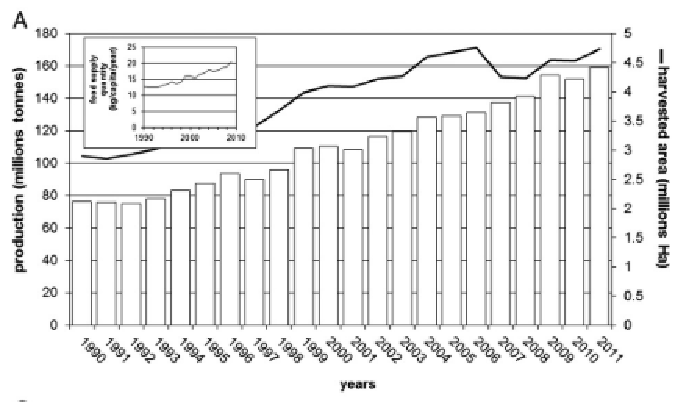
\includegraphics[width=.8\textwidth]{tomato_metrics_per_year}
 \tiny{\caption{Tomato production worldwide. Reprinted from Bergougnoux, V. (2014). The history of tomato: From domestication to biopharming. Biotechnology Advances.}}
\end{figure}
\end{frame} 

\begin{frame}{Context}{\tiny{Tomato production}}
 \begin{figure}
 \centering
 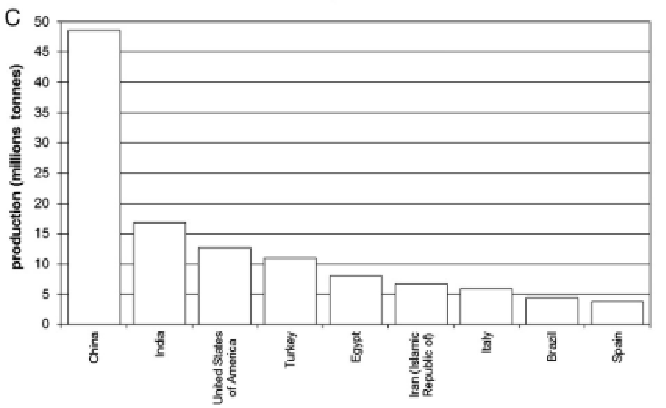
\includegraphics[width=.75\textwidth]{tomato_metrics_per_country}
 \tiny{\caption{Tomato production per country. Reprinted from Bergougnoux, V. (2014). The history of tomato: From domestication to biopharming. Biotechnology Advances.}}
\end{figure}
\end{frame}


\begin{frame}{Problem}
  
%\begin{block}{objetivo General}
Diseases and pests in tomato crop, and the development of non-invasive systems for its early detection that mitigate the food security.
%\end{block}
\end{frame}

\begin{frame}{Objectives}
 \begin{block}{General objective}
 Evaluation of different algorithms for anomaly
detection, in the context of tomato images.
 \end{block}
\end{frame}


\begin{frame}{Objetives}{\tiny{Specific objectives}}
  
  \begin{itemize}
  \item To design a dataset to train the machine learning models.
  \item Selection of an anomaly detection algorithms.
  \item To evaluate the selected methods for detection anomaly in tomato images.
  \end{itemize}
\end{frame}


\section{Solution}

\subsection{Anomaly detection with generative adversarial networks}


\begin{frame}{Anomaly detection with generative adversarial networks}{\tiny{Generative Adversarial Networks architecture}}
  % Coloque el diagrama de bloques detallado de su solución
  \begin{figure}
   \centering
   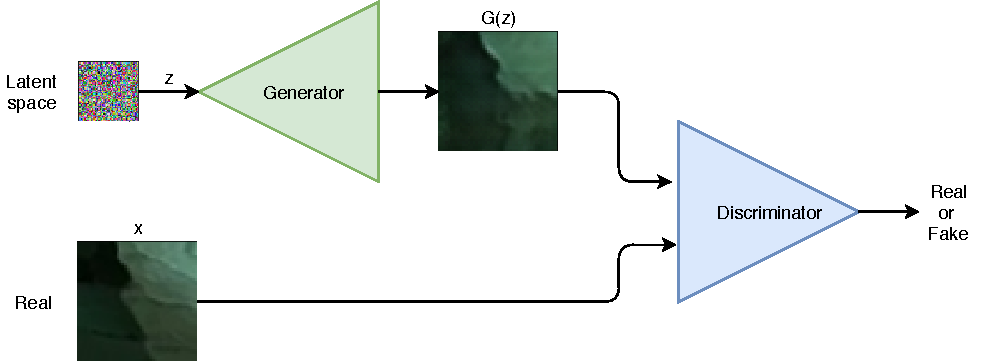
\includegraphics[width=\textwidth]{gan}
  \end{figure}
  
  \begin{equation}
  \nonumber
 \min _{G} \max _{D} V(D, G)=\mathbb{E}_{x \sim p_{\text {data }}(x)}[\log D(x)]+\mathbb{E}_{z \sim p_{z}(z)}[\log (1-D(G(z)))]
\end{equation}
\end{frame}

\begin{frame}{Anomaly detection with generative adversarial networks}{\tiny{Adversarial Anomaly Detector architecture}}
  % Coloque el diagrama de bloques detallado de su solución
  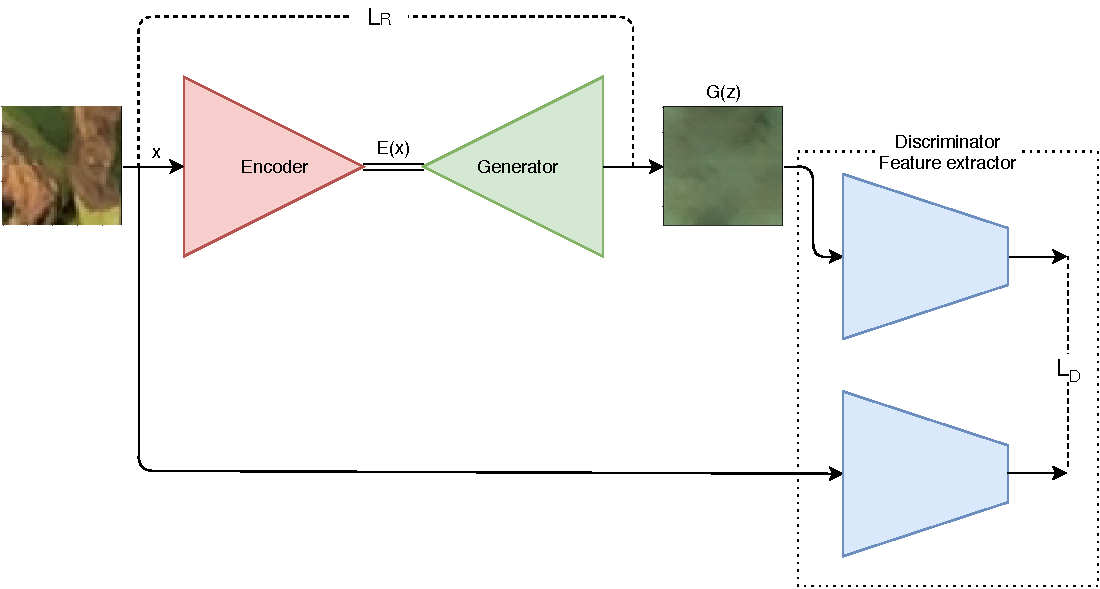
\includegraphics[width=\textwidth]{adversarial_anomaly_detector}
\end{frame}

\begin{frame}{Anomaly detection with generative adversarial networks}{\tiny{Adversarial Anomaly Detector loss function}}
 \begin{equation}
 \nonumber
 \mathcal{L}\left(\mathbf{E}(x)\right)=(1-\lambda) \cdot \mathcal{L}_{R}\left(\mathbf{E}(x)\right)+\lambda \cdot \mathcal{L}_{D}\left(\mathbf{E}(x)\right)
\end{equation} 

where the reconstruction error $\mathcal{L}_{R}$ and the discriminator error $\mathcal{L}_{D}$ are defined as follows:

\begin{equation}
 \nonumber
 \mathcal{L}_{R}\left(\mathbf{E}(x)\right)=\left\|\mathbf{x}-G\left(\mathbf{E}(x)\right)\right\|
\end{equation}

\begin{equation}
 \nonumber
 \mathcal{L}_{D}\left(\mathbf{E}(x)\right)=\left\|\mathbf{f}(\mathbf{x})-\mathbf{f}\left(G\left(\mathbf{E}(x)\right)\right)\right\|
\end{equation}

\end{frame}

\section{Results}

\begin{frame}{GAN training}
  \begin{figure}
   \centering
   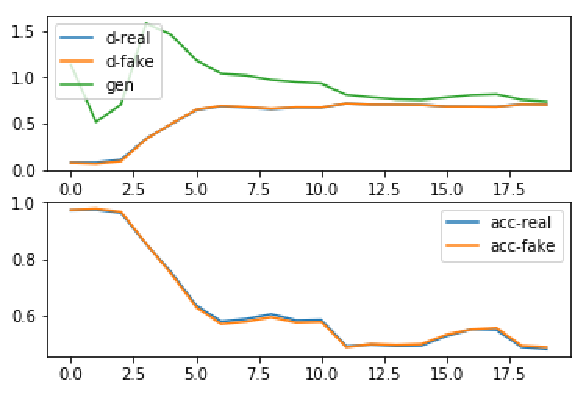
\includegraphics[width=.75\textwidth]{gan_training}
  \end{figure}
\end{frame}

\begin{frame}{GAN training}
 
 
\begin{figure}[H]
\centering
\begin{minipage}{.5\textwidth}
  \centering
  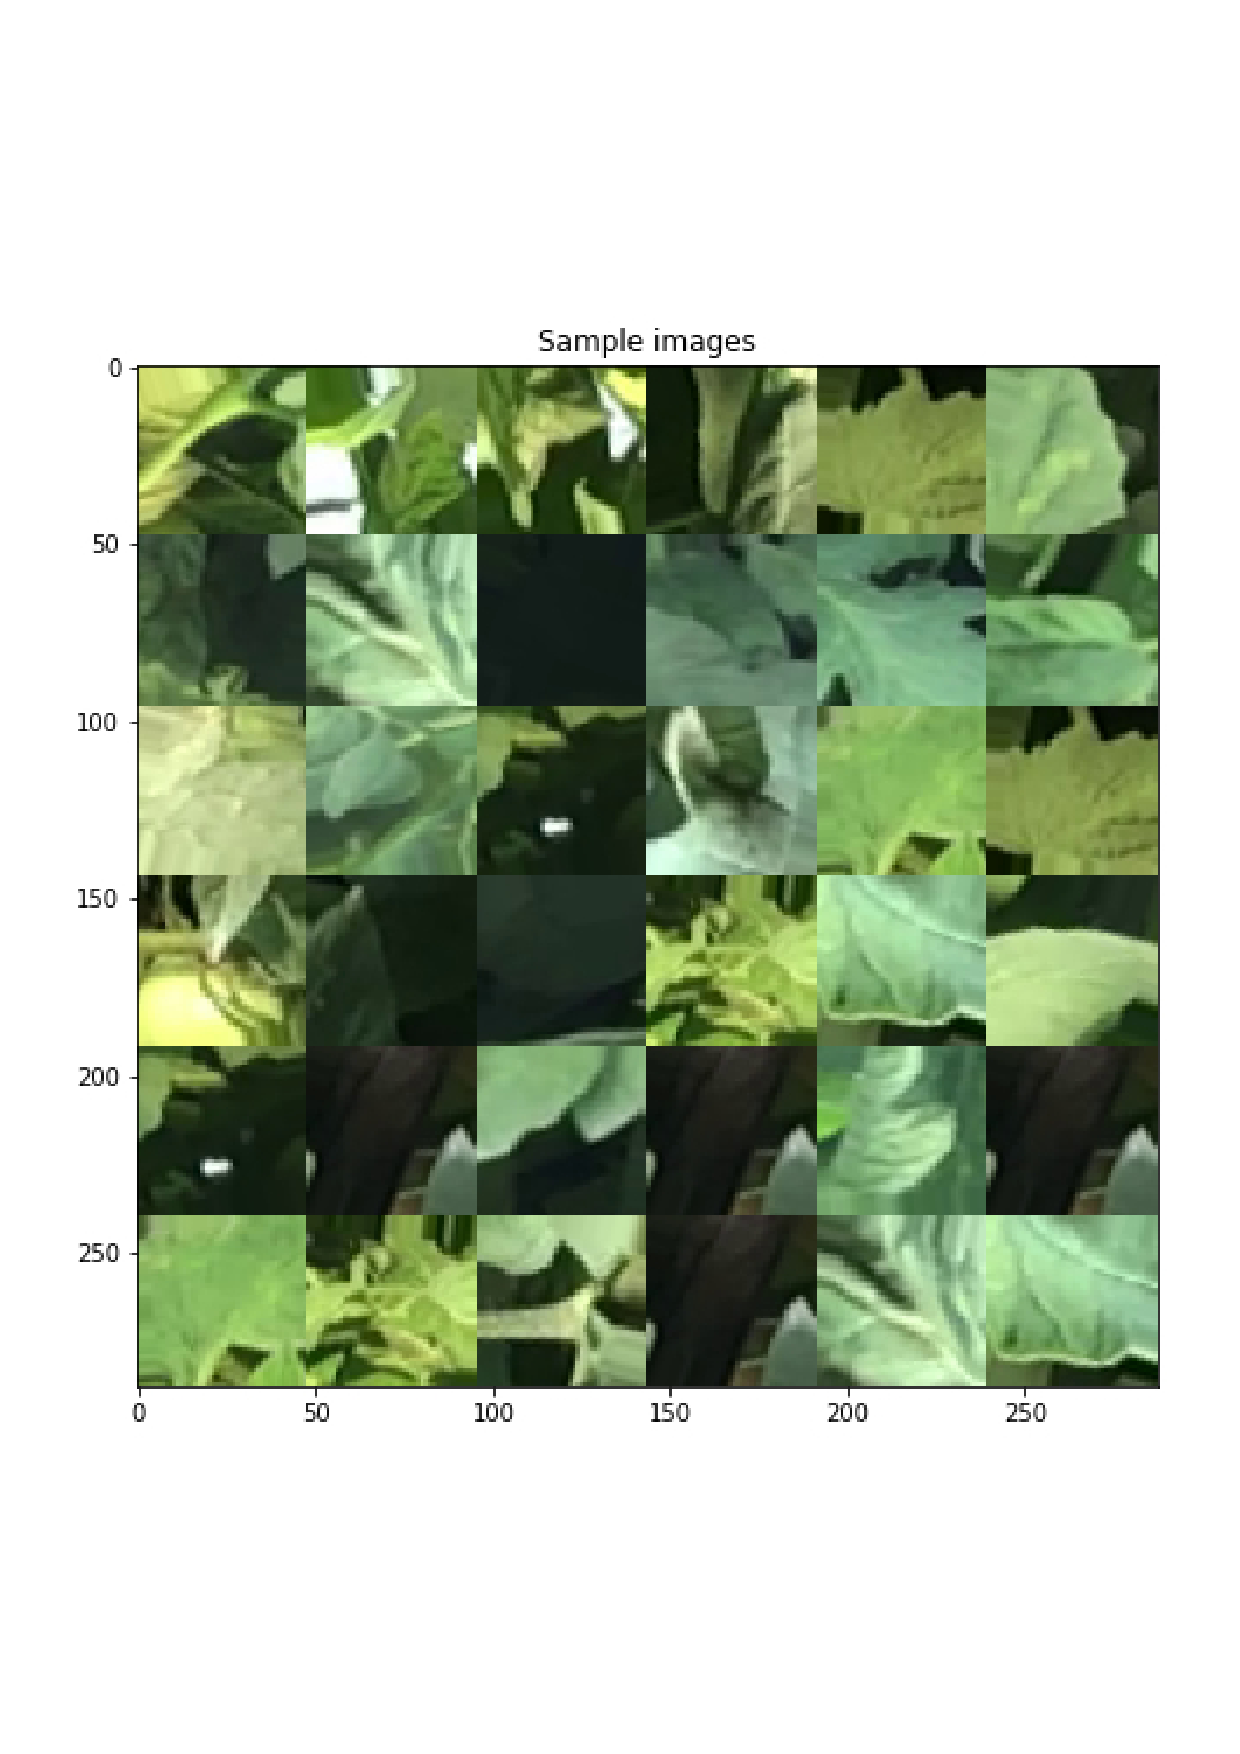
\includegraphics[width=.75\linewidth]{samples}
\end{minipage}%
\begin{minipage}{.5\textwidth}
  \centering
  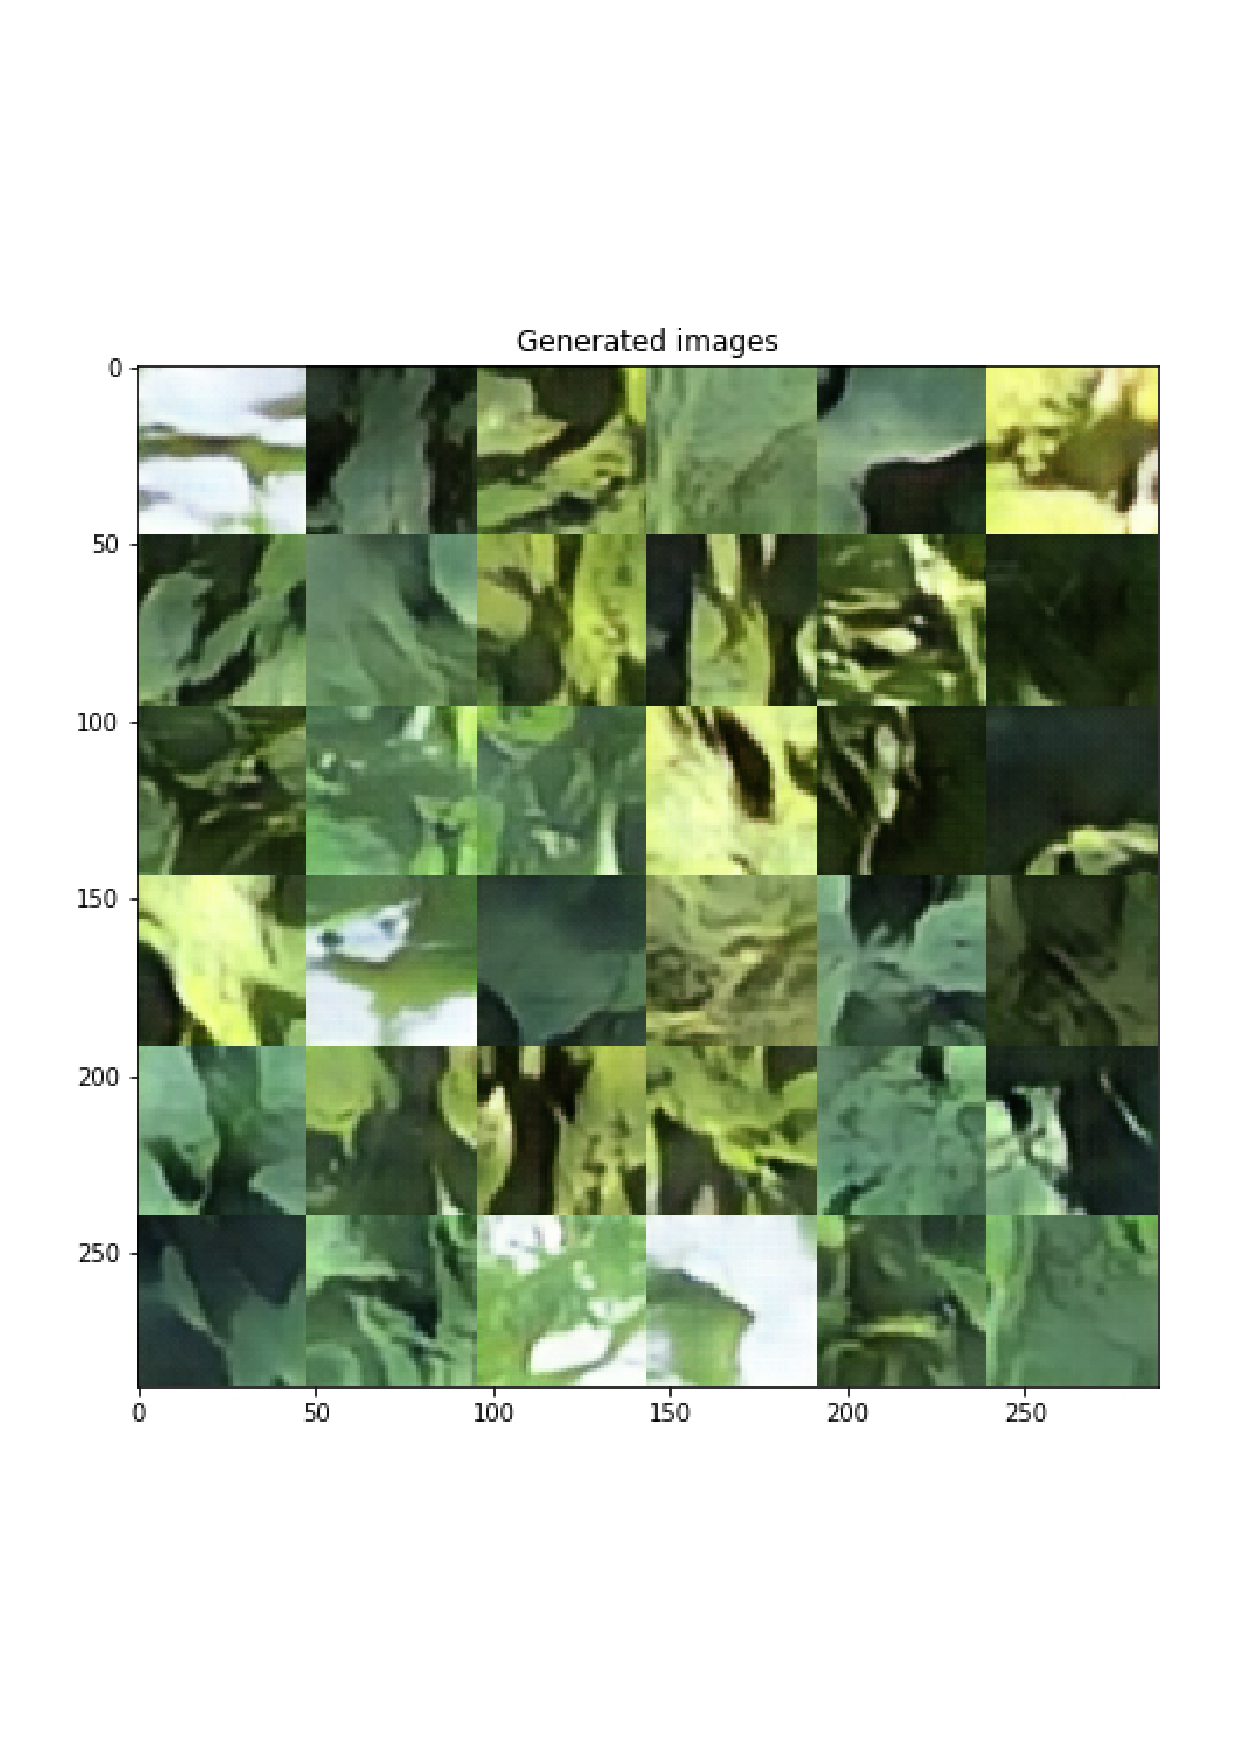
\includegraphics[width=.75\linewidth]{generated_samples}
\end{minipage}
\end{figure}
 
 
\end{frame}


\begin{frame}{Reconstruction evaluation}
 \begin{table}
    \centering
    \caption[Reconstruction metric evaluation]{Reconstruction metric evaluation.}
    \begin{tabular}{ c c c c c }
        \hline
        Model & Mean & STD & Mean & STD \\
        & (healthy) & (healthy) & (anomalies) & (anomalies) \\
        \hline
        sVAE & 10410.6 & 7020.3 & 19858.8 & 18464.1 \\
        GM-VAE & 15162.2 & 7597.3 & 9357.3 & 6071.7 \\
        AAD & 3839.5 & 3251.1 & 8996.1 & 3308.8 \\
        \hline
    \end{tabular}
\end{table}
\end{frame}


\begin{frame}{Reconstruction evaluation}
 \begin{table}[htb]
    \caption[Reconstruction time evaluation]{Reconstruction time evaluation.}
    \label{table:rec_time}
    \centering
    \begin{tabular}{ c c c }
        \hline
        Model & Reconstruction time (ms) \\
        \hline
        sVAE & 160.8 \\
        GM-VAE & 1383.1 \\
        AnoGAN & 6320.6 \\
        Adversarial Anomaly Detector & 255.3 \\
        \hline
    \end{tabular}
\end{table}
\end{frame}

\begin{frame}{Reconstruction evaluation}
 \begin{figure}
   \centering
   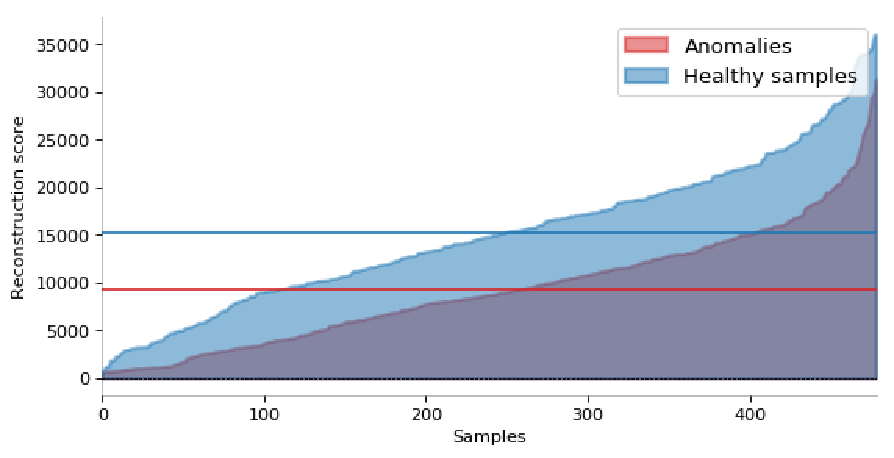
\includegraphics[width=.85\textwidth]{rec_gmvae_eval}
  \end{figure}
\end{frame}

\begin{frame}{Reconstruction evaluation}
 \begin{figure}
   \centering
   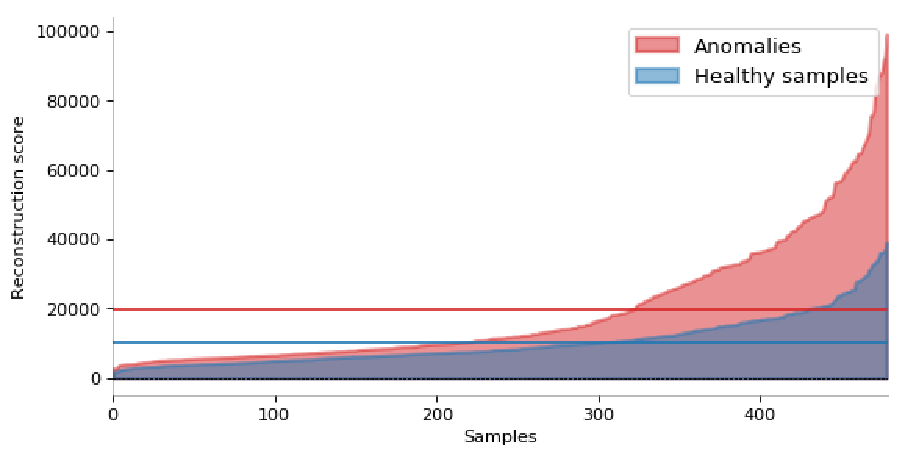
\includegraphics[width=.85\textwidth]{rec_svae_eval}
  \end{figure}
\end{frame}

\begin{frame}{Reconstruction evaluation}
 \begin{figure}
   \centering
   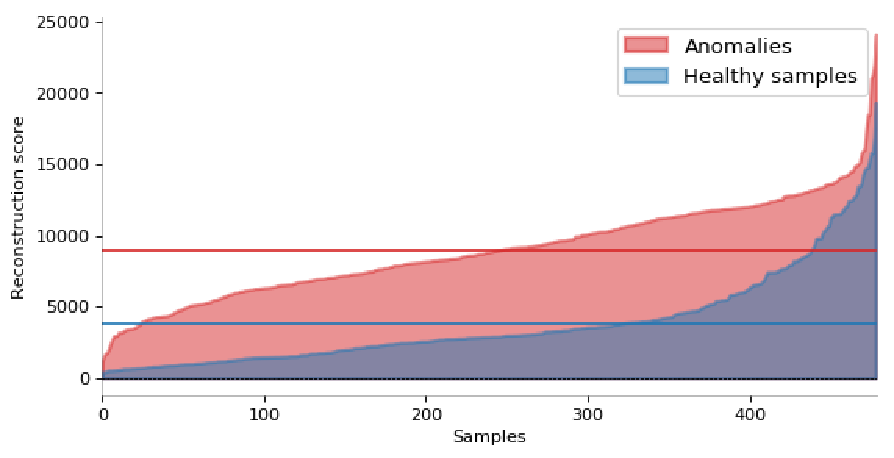
\includegraphics[width=.85\textwidth]{rec_anogan_eval}
  \end{figure}
\end{frame}

\begin{frame}{t-SNE evaluation}
 \begin{figure}
  \centering
  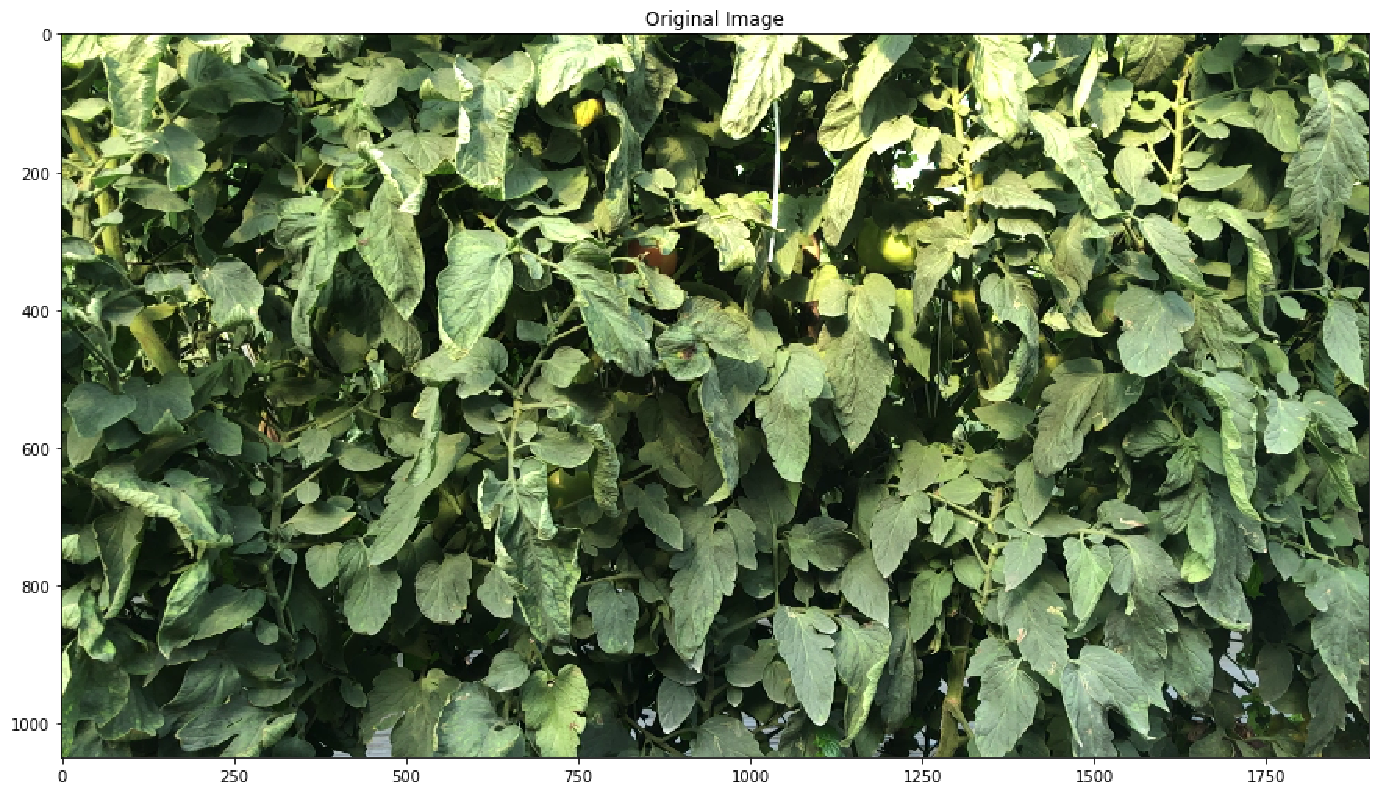
\includegraphics[width=.85\textwidth]{anogan_test_image1}
  \caption{Test image with regular samples}
 \end{figure}
\end{frame}

\begin{frame}{t-SNE evaluation}
 \begin{figure}
  \centering
  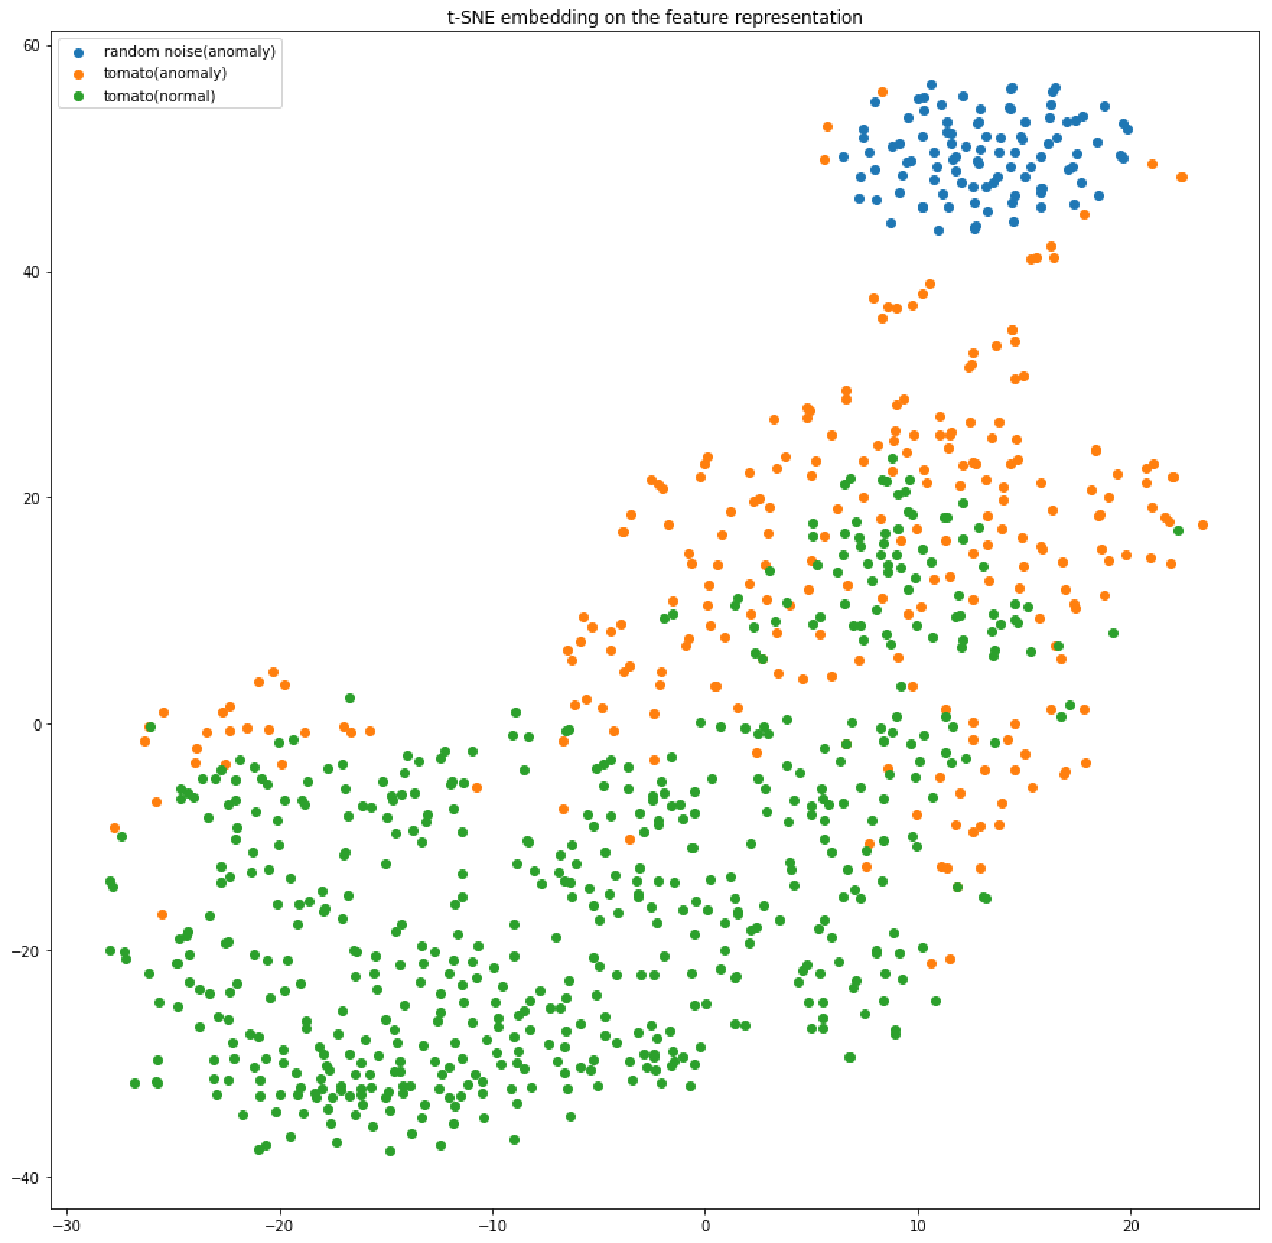
\includegraphics[width=.6\textwidth]{anogan_t_sne1}
 \end{figure}
\end{frame}

\begin{frame}{t-SNE evaluation}
 \begin{figure}
  \centering
  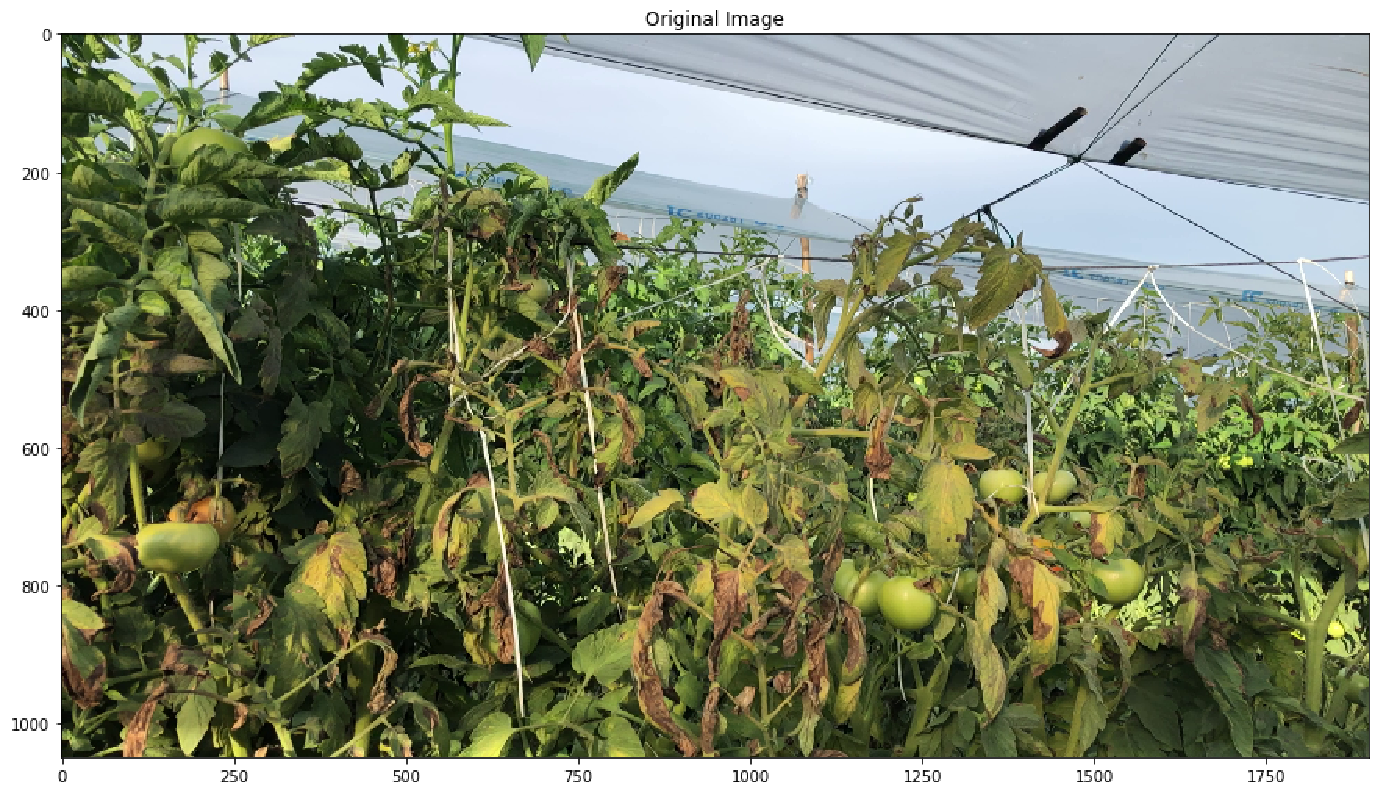
\includegraphics[width=.85\textwidth]{anogan_test_image2}
  \caption{Test image with anomalous samples}
 \end{figure}
\end{frame}

\begin{frame}{t-SNE evaluation}
 \begin{figure}
  \centering
  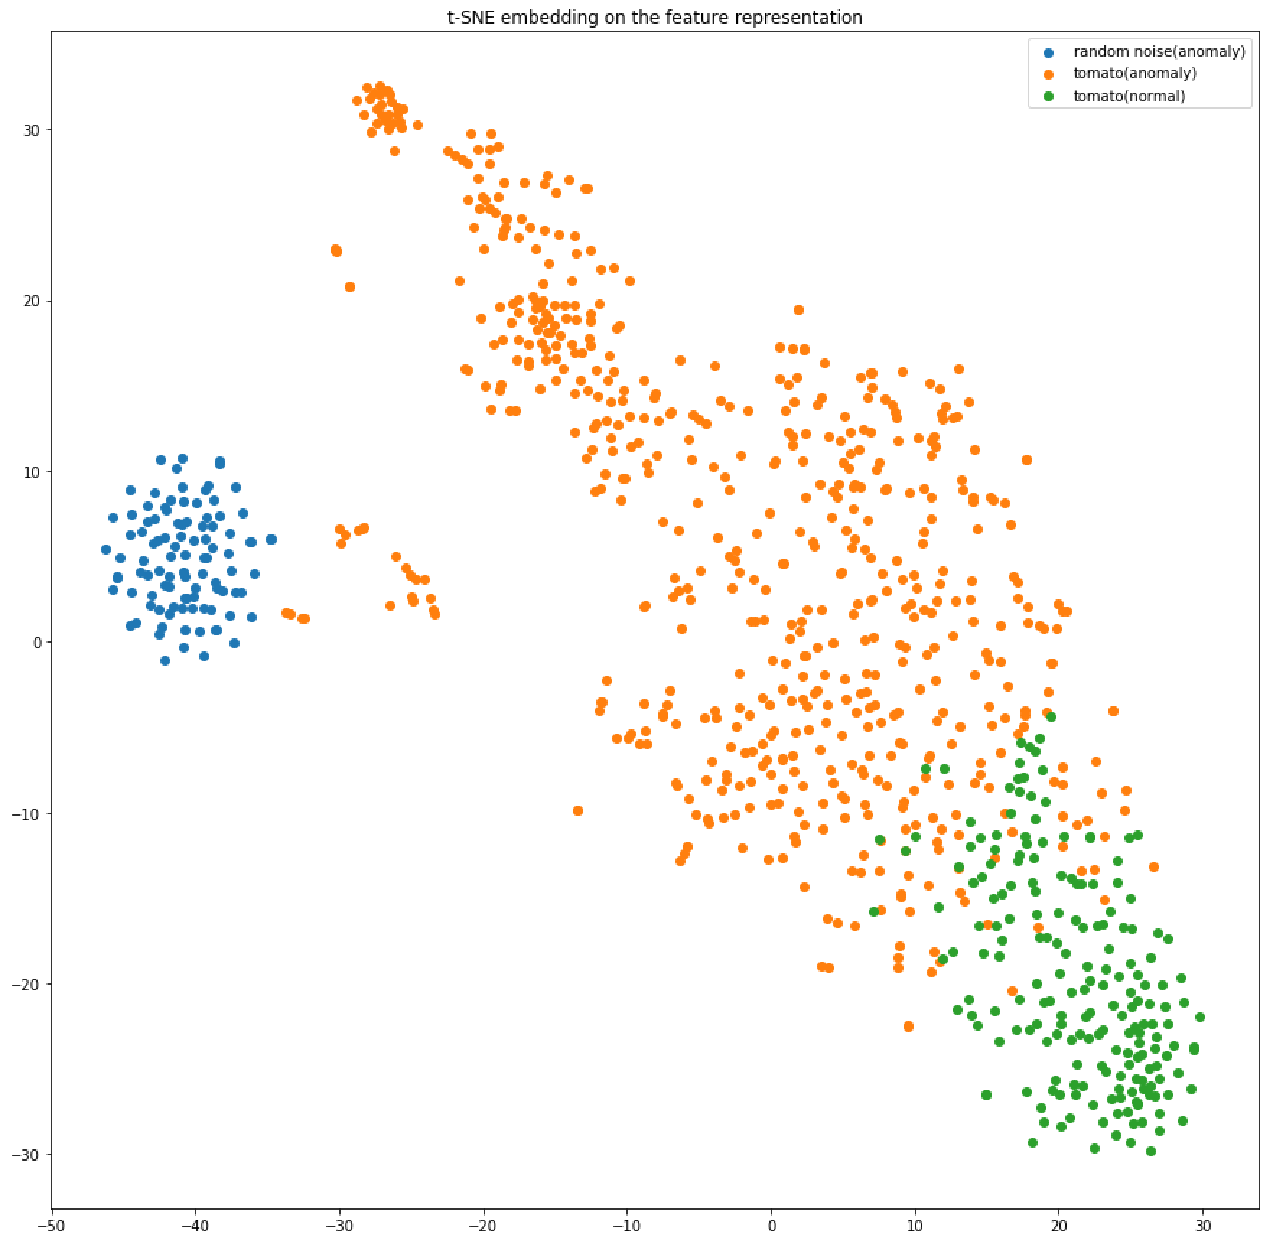
\includegraphics[width=.6\textwidth]{anogan_t_sne2}
 \end{figure}
\end{frame}

\begin{frame}{Conclusions}
  
  \begin{itemize}
  \item The experiments performed so far have shown a tendency of the variational autoencoder
architectures to blur the reconstructed image
  \item  The GAN-based architectures have more
promising results with better reconstruction images
  \item A modification to the AnoGAN architecture is proposed, allowing to considerably improve
the reconstruction time
  \end{itemize}
  
\end{frame}

\begin{frame}{Future work}
  
  \begin{itemize}
  \item Improve the generator of the GAN
  \item Metrics that evaluate the GAN performance needs to be explored, along with more metrics for the evaluation of the anomaly detections
  \item A segmentation process should be implemented in order to mark possible anomalous regions
  \end{itemize}
  
\end{frame}


\section{Summary}

\begin{frame}{Summary}
  \tableofcontents
\end{frame}

\end{document}
